% A simple Pentagon with TiKZ
% Author: Christoph Gerum <gerum@informatik.uni-tuebingen.de>

\documentclass{article}

\usepackage{tikz}


\begin{document}

%circle
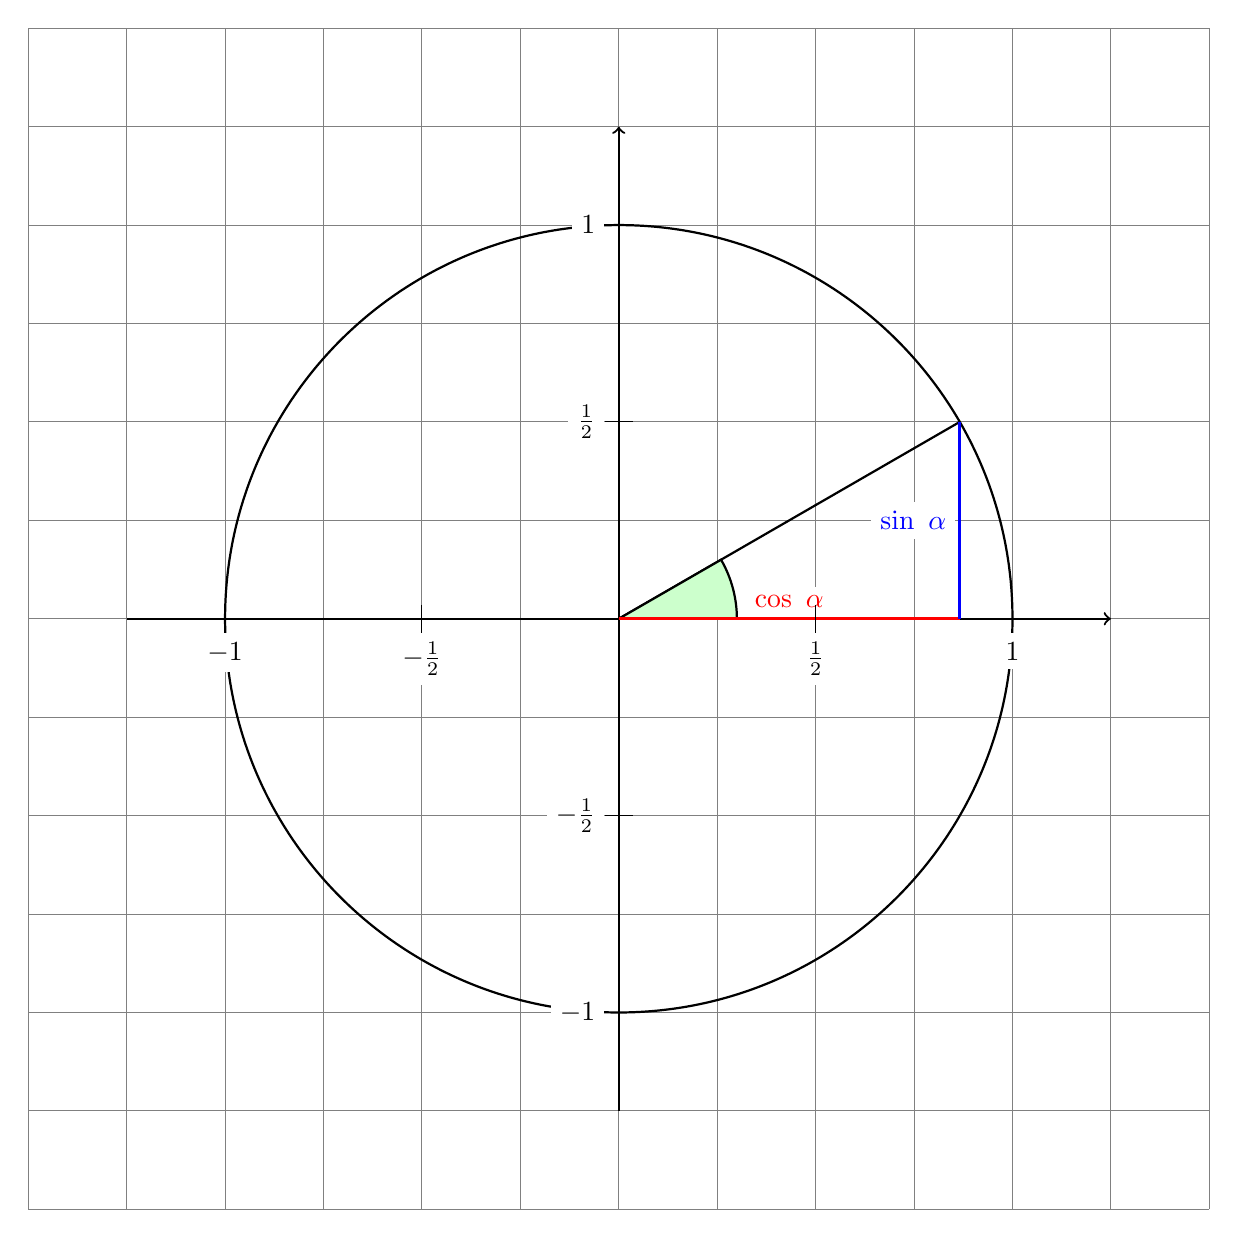
\begin{tikzpicture}[scale=5.0]
  \draw [step=0.25cm,color=gray] (-1.5, -1.5) grid (1.5, 1.5);
  
  \draw[->,thick] (-1.25, 0) -- (1.25,0);
  \draw[->,thick] (0,-1.25) -- (0,1.25);

  \draw[thick] (0,0) circle (1);
  \draw[thick] (0,0) -- (30:1cm);

  \filldraw[thick,fill=green!20]        (0,0) -- (0.3,0) arc (0:30:0.3) -- cycle;

  \draw[very thick, color=red]   (0,0)  -- node[anchor=south,fill=white]{$\cos\ \alpha$} (0,0 -| 30:1cm);
  \draw[very thick, color=blue]  (30:1cm) -- node[left=1pt,fill=white]{$\sin\ \alpha$} (0,0 -| 30:1cm);

  \foreach \x/\xtext in {1/1, 0.5/\frac{1}{2}, -0.5/-\frac{1}{2}, -1/-1}{
    \draw (\x,1pt) -- (\x, -1pt) node[anchor=north, fill=white]{$\xtext$};
    \draw (1pt, \x) -- (-1pt, \x) node[anchor=east, fill=white]{$\xtext$};
  }

\end{tikzpicture}


\end{document}
